 \documentclass[conference]{IEEEtran}
\IEEEoverridecommandlockouts
% The preceding line is only needed to identify funding in the first footnote. If that is unneeded, please comment it out.
\usepackage{cite}
\usepackage{amsmath,amssymb,amsfonts}
\usepackage{algorithmic}
\usepackage{graphicx}
\usepackage{float} 
\usepackage{subfigure} 
\usepackage{textcomp}
\usepackage{xcolor}
\def\BibTeX{{\rm B\kern-.05em{\sc i\kern-.025em b}\kern-.08em
    T\kern-.1667em\lower.7ex\hbox{E}\kern-.125emX}}
\begin{document}

\title{Implementation and Deployment: Tripedia\\
}

\author{\IEEEauthorblockN{Yulin Zhang}
\IEEEauthorblockA{\textit{7th Group} \\
\textit{Software Engineering}\\
Montreal, Canada \\
silveralex2023820@gmail.com}
\and
\IEEEauthorblockN{Yuhang Chen}
\IEEEauthorblockA{\textit{7th Group} \\
\textit{Software Engineering}\\
Montreal, Canada \\
yuhang.chen@mail.concordia.ca}
\and
\IEEEauthorblockN{Jiaxi Yang}
\IEEEauthorblockA{\textit{7th Group} \\
\textit{Software Engineering}\\
Montreal, Canada \\
yjxyang2@outlook.com}
\and
\IEEEauthorblockN{Boyang Wang}
\IEEEauthorblockA{\textit{7th Group} \\
\textit{Software Engineering}\\
Montreal, Canada \\
wangboyang0626@outlook.com}
}

\maketitle






\begin{figure*}[htbp]
\centerline{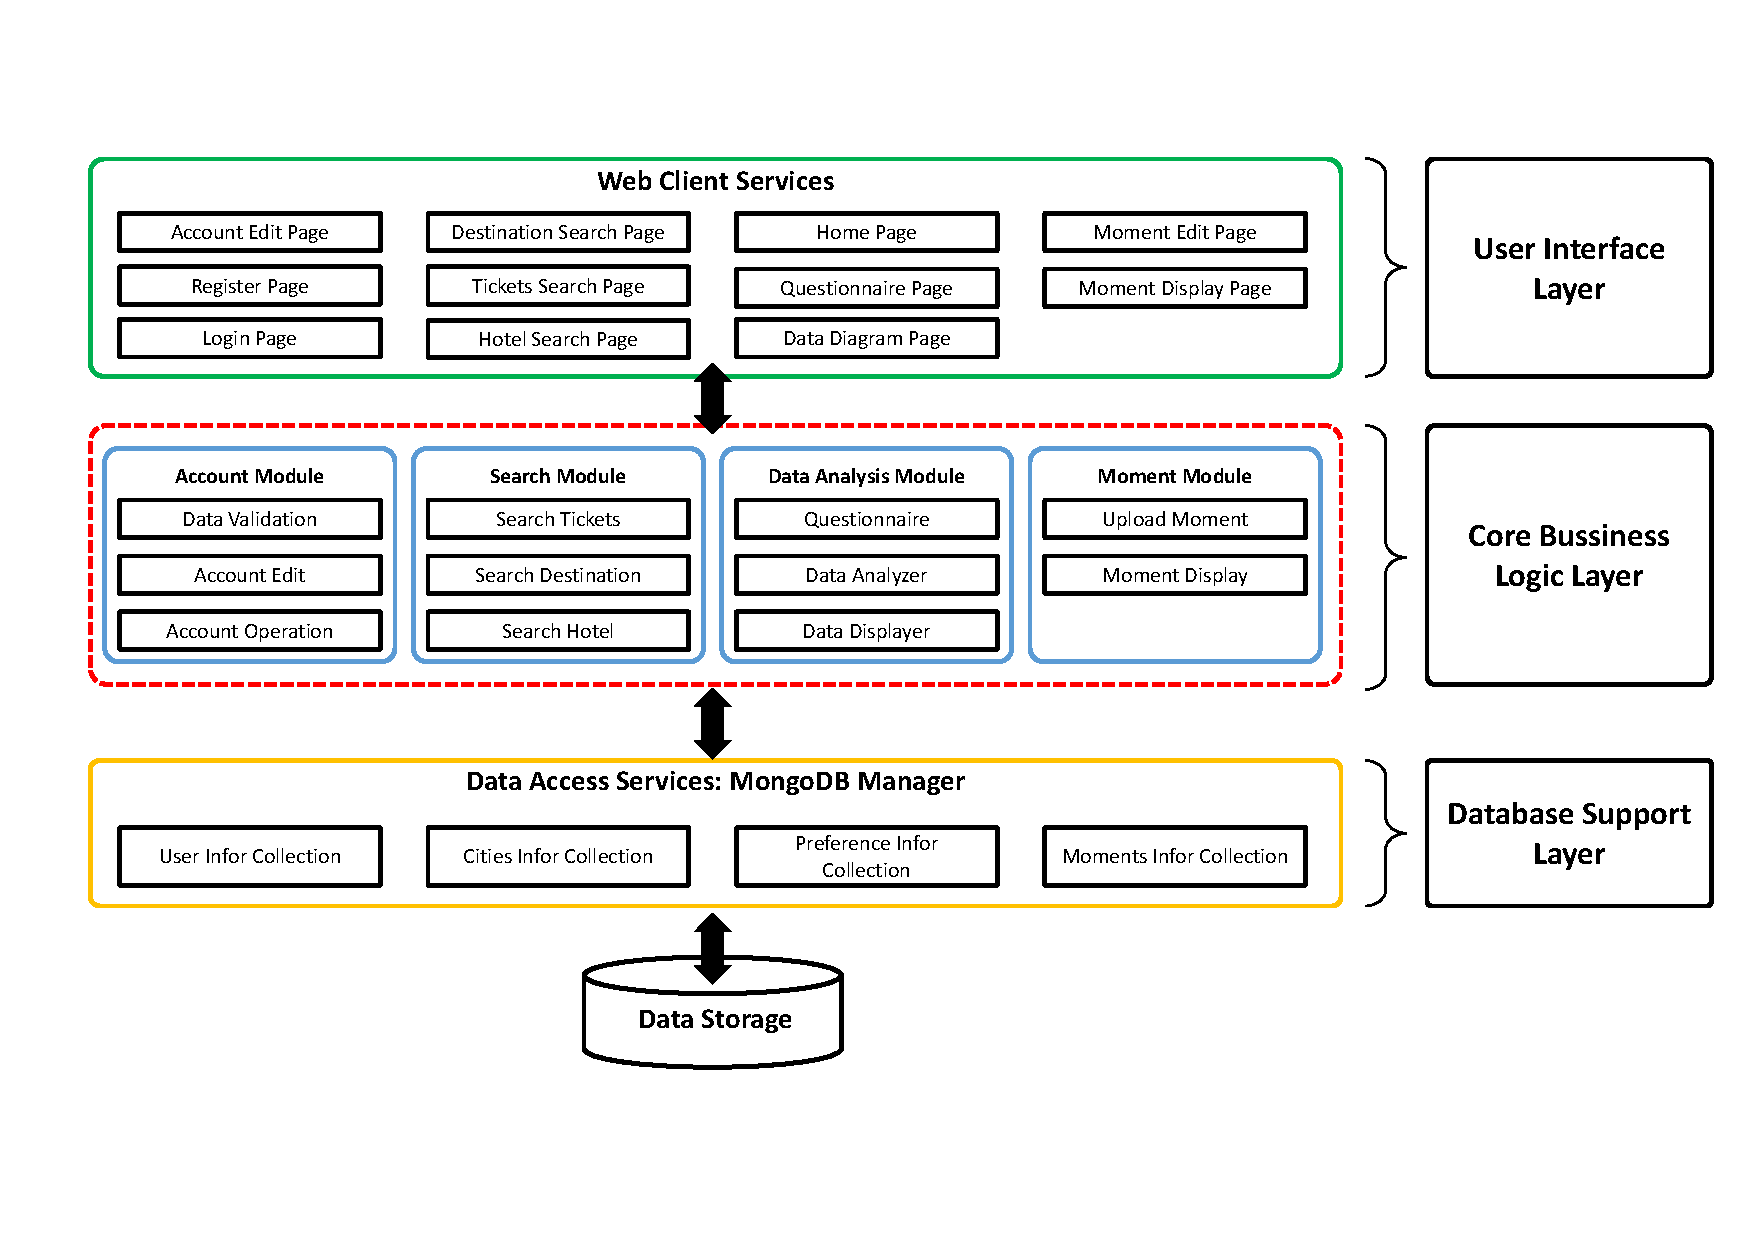
\includegraphics[width=1.0\textwidth]{Architecture2.pdf}}
\caption{The Adoption of Layered Architecture Pattern in Tripedia.}
\label{system_architecture_layered}
\end{figure*}

\begin{table*}[htbp]
\caption{The software metrics and granularity of components.}
\begin{center}
\begin{tabular}{|c|c|c|c|}
\hline
\textbf{Task Name} & \textbf{\textit{LOC}}& \textbf{\textit{Component Granularity Level}}& \textbf{\textit{Numbers of Units}} \\
\hline
Account Login and Password Validation &  & Module & 1 \\
Data Displayer &   & Python Class & 1 \\
Data Analyzer &  & Python Class &  1 \\
Questionnaire &  & Module & 1 \\
\hline
\end{tabular}
\label{tab1}
\end{center}
\end{table*}



\section{\textbf{Architectural Design Process}}

\textbf{Question: Identify and articulate what are your architectural designs and the associated
software engineering process.}

Architectural designs serve as the blueprints for our software systems, shaping their form and defining the relationships among components. Our design choice comes with its own set of considerations and implications. In chapter, we will dissect the architectural design in Tripedia system.


\subsection{\textbf{Architectural Design}}

\subsection{\textbf{Software Engineering Process}}


\section{\textbf{Architecture Design Consideration}}

\textbf{Question: Indicate if any revision to your architectural design is necessary. If the answer is Yes, please explain what revision, and the reason.}

In this chapter, we will explore the senarios about our system. And we will give reasons about our descision about revision.

\subsection{\textbf{Revision Consideration}}




\subsection{\textbf{Reasons}}

Adequate Initial Planning: The initial architectural design was thoroughly planned, considering all the key aspects of the project. This careful planning ensured that the architecture was well-suited to meet the project's requirements from the beginning.

Flexibility and Scalability: The chosen architecture was flexible and scalable, capable of accommodating the evolving needs of the project without requiring fundamental changes. This adaptability helped in avoiding major architectural revisions.

Proven Architectural Pattern: Employing a proven and tested architectural pattern (like MVC, for example) which is known for its reliability and efficiency in similar projects, reduced the need for changes.

Consistent Project Requirements: There were no significant changes in the project requirements or scope that necessitated a revision of the architectural design. The consistency in requirements helped in maintaining the original architecture.
Effective Risk Management: Potential risks and challenges were identified and mitigated early in the development process, which prevented any architectural disruptions.

Regular Reviews and Feedback: Continuous monitoring and regular reviews of the architecture ensured that any minor issues were addressed promptly, eliminating the need for major revisions.

Team Expertise and Experience: The experience and expertise of the development team in working with the chosen architecture led to efficient problem-solving and decision-making, keeping the architecture stable and effective.

Technological Compatibility: The selected technology stack and tools were fully compatible with the chosen architecture, ensuring smooth development and operation processes.

By providing these reasons, you're effectively communicating that the initial architectural choice was sound and remained relevant and effective throughout the development process.



\section{\textbf{The Adoption of MVC and Layered Architecture}}

\textbf{Question: Further adopt MVC and Layered Architecture Pattern to your ICDE-App. Describe your design
decisions, and discuss the pros and cons of the design.}

In this chapter, we discuss the adoption of MVC and Layered Architecture Patterns into Tripedia system. By embracing these architectural patterns, we aim to achieve a balance between flexibility, scalability, and maintainability. Finally, we explain the pros and cons of our system architecture.


\subsection{\textbf{The Adoption of MVC Architecture Pattern}}


\subsection{\textbf{The Adoption of Layered Architecture Pattern}}


\subsection{\textbf{The Pros and Cons}}






\section{\textbf{Software Metrics and Granularity of Components}}

\textbf{Question: Please make a statistical count of software metrics from all your tasks implemented so far and
form a table given the template below. }










\end{document}
